\section{Einleitung}\raggedbottom
\label{sec:1}
Im Folgenden Abschnitt werden zunächst einmal Grammatiken und Automaten definiert und anhand eines kurzen Beispiels erläutert. Die hier verwendeten Definitionen sind an das Drachenbuch\cite{DraBu} angelehnt.
\subsection{Grammatiken}
\label{sec:1.1}
Eine Grammatik setzt sich aus den vier folgenden Bestandteilen zusammen:
\begin{itemize}
	\item Einer Menge von Terminalen. Terminale sind die Symbole, welche die von der Grammatik erzeugten Sprache ausmachen.
	\item Einer Menge von Nichtterminalen. Jedes Nichtterminal wird mit einer Produktion auf eine Liste von weiteren Terminalen und Nichtterminalen abgebildet, so dass durch wiederholte Anwendung dieser Produktionen Terminalstrings (Wörter) entstehen.
	\item Einer Menge von Produktionen. Eine Produktion hat drei Bestandteile: Ein Nichtterminal auf der linken Seite, einen Pfeil in der Mitte und eine Reihe von Terminalen und Nichtterminalen auf der rechten Seite. Die Produktionen beschreiben wie die Terminale und Nichtterminale zu Wörtern zusammengesetzt werden, die nur noch Terminale enthalten.
	\item Einem Startsymbol. Eines der Nichtterminale wird als Startsymbol ausgewiesen. Bei der Bildung eines Wortes wird immer mit einer der Regeln des Startsymbols begonnen.
\end{itemize}
Ein Beispiel für eine Grammatik wäre:
\lstset{
	captionpos=b,
	breaklines=true,
}
\begin{lstlisting}[frame=single, caption=Beispiel für eine Grammatik]
{a, b; S, A; S}

S --> aA
A --> aA
A --> b
\end{lstlisting}
Diese Grammatik besteht aus den Terminalen a und b, den Nichtterminalen S und A, wobei S das Startsymbol der Grammatik ist, und den drei aufgelisteten Produktionen. Die von dieser Grammatik erzeugten Wörter sind sehr einfach:\\
Man beginnt mit dem Startsymbol S und leitet es nach aA ab. Anschließend kann man das A beliebig oft nach aA ableiten und um das Wort abzuschließen leitet man es einmal nach b ab. Es entstehen also Wörter wie zum Beispiel \textit{ab}, \textit{aab}, \textit{aaaaaab}, etc.
\subsection{Automaten}
\label{sec:1.2}
Bei Automaten unterscheiden wir zwischen deterministischen und nichtdeterministischen endlichen Automaten. Diese beiden Formen von Automaten sind sich sehr ähnlich: Deterministische Automaten weisen jedoch eine bedeutende Einschränkung im Vergleich zu nichtdeterministischen Automaten auf. Beide sind Akzeptoren, das heißt sie können ein Eingabewort entweder akzeptieren oder nicht.
\\
Ein nichtdeterministischer endlicher Automat (NFA) besteht aus:
\begin{itemize}
	\item Einer endlichen Menge von Zuständen
	\item Einer Menge von Eingabesymbolen (dem Eingabealphabet). Diese entsprechen den Terminalsymbolen bei einer Grammatik.
	\item Einer Übergangsfunktion, die für jeden Zustand und jedes Symbol aus dem Eingabealphabet eine Menge von nächsten Zuständen ausgibt.
	\item Einem Startzustand. Hierzu wird ein Zustand des Automaten als Startzustand ausgewiesen.
	\item Einer Menge von Endzuständen. Wenn die Übergangsfunktion für ein bestimmtes Eingabewort einen dieser Zustände ausgibt, wird das Wort vom Automaten akzeptiert.
\end{itemize}
Ein deterministischer endlicher Automat (DFA) besteht aus den gleichen Komponenten. Jedoch muss die Übergangsfunktion hier für einen Zustand und ein Eingabesymbol aus dem Eingabealphabet nur genau einen nächsten Zustand ausgeben, im Gegensatz zu einem NFA, bei dem sie eine Menge von Zuständen ausgibt, die auch leer sein kann.\\
NFAs und DFAs können durch einen gerichteten Graph dargestellt werden. Die Knoten dieses Graphen sind die Zustände des jeweiligen Automaten und die Kanten stehen für seine Übergangsfunktion. Man nennt diesen Graph \textit{Übergangsgraph}.\\
Der folgende Automat mit dem Eingabealphabet \{a, b\} und der Zustandsmenge \{z0, z1, z2\} akzeptiert die von der oben gezeigten Grammatik erzeugte Sprache.
\begin{figure}[H]
	\centering
	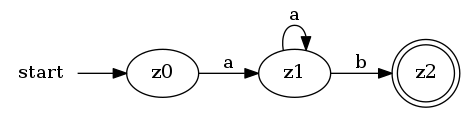
\includegraphics[width=0.75\textwidth]{bilder/beispiel_automat1.png}
	\caption{Beispiel für einen DFA}
	\label{fig:pic1}
\end{figure}
Wie man erkennt, wird z0 durch einen Startpfeil als Startzustand und z2 durch einen doppelten Kreis als Endzustand markiert.